\section{Μεθοδολογία}
\label{Methodology}

Στο κεφάλαιο αυτό παρουσιάζεται αναλυτικά η δομή και ο τρόπος λειτουργίας του προτεινόμενου συστήματος. Ο τρόπος εκπαίδευσης του συστήματος παρουσιάζεται στο κεφάλαιο \ref{Training}. Συμπεριλαμβάνονται επακριβείς πληροφορίες για την προεπεξεργασία των δεδομένων, τη δομή του μοντέλου και για το post-processing που εφαρμόζεται.

\subsection{Προεπεξεργασία Δεδομένων}
\label{DataPreprocessing}

Η προεπεξεργασία των δεδομένων αποτελεί βασικό τμήμα κάθε μελέτης στη Βαθιά Μάθηση. Αποτελεί τη διαδικασία κατά την οποία τα δεδομένα, τα οποία αρχικά βρίσκονται σε μορφή που δεν μπορούν να υποστηρίξουν μάθηση (στην περίπτωσή μας, τα αρχικά βίντεο των ομιλητών με τον ήχο), αποκτούν τη μορφή που τους επιτρέπει να εισαχθούν στο μοντέλο. Αξιοποιώντας τις γνώσεις πάνω στο αντικείμενο, είναι δυνατόν να μειωθεί ο χρόνος εκπαίδευσης μέσω της μείωσης των διαστάσεων των πληροφοριών που εισάγονται στο νευρωνικό δίκτυο και, γενικότερα, να βελτιωθούν τα τελικά αποτελέσματα. Παρακάτω αναλύονται οι εκάστοτε τεχνικές pre-processing που εφαρμόζονται ώστε να λάβουν τα δεδομένα την επιθυμητή μορφή.

\subsubsection{Εξαγωγή της περιοχής των χειλιών}
\label{LipExtraction}
Έστω ένα βίντεο ομιλητή $T \times C \times H \times W$ με $T$ τη χρονική διάσταση (τον αριθμό των frames), $C$ τον αριθμό των καναλιών (για RGB βίντεο είναι 3) και $H$ ύψος και $W$ πλάτος σε pixel. Για να περιοριστεί το μέγεθος των δεδομένων και να παραλειφθούν περιττές πληροφορίες του παρασκηνίου αλλά και του προσώπου του ομιλητή, αναπτύχθηκε ένα pre-processing script εντοπισμού της περιοχής των χειλιών. Η περιοχή αυτή είναι που αφορά το αντικείμενο, καθώς εκεί βρίσκεται η πληροφορία των visemes (άλλωστε, για αυτό αποκαλείται lip reading). Χρησιμοποιώντας το διαθέσιμο προεκπαιδευμένο MediaPipe Face Landmarker της Google, εντοπίζονται τα διάφορα ``τοπόσημα προσώπου'' (facial landmarks) του ομιλητή για κάθε frame του αρχικού βίντεο. Οι δείκτες των τοποσήμων των χειλιών εξάγονται για κάθε frame ξεχωριστά και παράγουν μία νέα εικόνα της περιοχής αυτής με διαστάσεις $H' \times W' \times 3$ και $H'<H, W'<W$. Συγκεκριμένα, υπολογίζεται το ελάχιστο ορθογώνιο (bounding box) που περιέχει όλα τα τοπόσημα των χειλιών, το οποίο διευρύνεται για ασφάλεια (padding) κατά 30\% του πλάτους του σε κάθε οριζόντια πλευρά και κατά 30\% του ύψους του σε κάθε κατακόρυφη πλευρά, χωρίς να ξεπερνά τα όρια του frame. Έτσι, η περιοχή που αποκόπτεται έχει περίπου 1.6 φορές το πλάτος και 1.6 φορές το ύψος των χειλιών.

Από τα εκάστοτε frames παράγεται το νέο βίντεο της περιοχής των χειλιών, κάθε frame του οποίου επαναδειγματοληπτείται (resampling με παρεμβολή τύπου area) στην προεπιλεγμένη τελική διάσταση $224 \times 224$, δίνοντας βίντεο διαστάσεων $224 \times 224 \times 3 \times T$. Η αλλαγή μεγέθους σε τετράγωνο δεν διατηρεί τον λόγο πλευρών της αρχικής περιοχής, η οποία είναι αισθητά πλατύτερη από ό,τι ψηλή, με αποτέλεσμα τα χείλη να εμφανίζονται κατακόρυφα τεντωμένα στην τελική εικόνα. Κατά τον εντοπισμό των τοποσήμων χρησιμοποιείται και ένας μηχανισμός fallback, σε περίπτωση που το Face Landmarker αδυνατεί να βρει τους ζητούμενους δείκτες. Συγκεκριμένα, εάν δεν εντοπιστούν για ένα δεδομένο frame τα τοπόσημα, τότε επαναχρησιμοποιούνται αυτά του προηγούμενου frame, ενώ αν δεν υπάρχουν ούτε αυτά εκτιμάται η τοποθεσία των χειλιών ως η κάτω περιοχή του προσώπου (50\% του πλάτους και 35\% του ύψους, με κατακόρυφο offset 42\%). Τα δεδομένα κωδικοποιούνται σε μορφή βίντεο .mp4 διατηρώντας το framerate του αρχικού βίντεο, ενώ παράγονται και μερικά παραδείγματα frames από το βίντεο bbaf2n.mpg του dataset GRID (βλ. παράγραφο \ref{Datasets}), τα οποία παρουσιάζονται παρακάτω.

Τα παραδείγματα αφορούν τέσσερα ισαπέχοντα frames του βίντεο (τα frames 0, 24, 49 και 74 από τα συνολικά 75). Σε κάθε σχήμα, αριστερά απεικονίζεται το αρχικό frame του GRID, διαστάσεων $360 \times 288$ pixels (πλάτος $\times$ ύψος), πάνω στο οποίο το πράσινο ορθογώνιο δείχνει την περιοχή που αποκόπτεται (το bounding box των χειλιών μαζί με το padding), ενώ δεξιά απεικονίζεται η εικόνα που προκύπτει από την περιοχή αυτή μετά την αλλαγή μεγέθους σε $224 \times 224$ pixels. Για λόγους παρουσίασης, στα σχήματα το αρχικό frame έχει κλιμακωθεί ώστε να έχει ύψος 256 pixels και η δεξιά εικόνα σε $256 \times 256$ pixels. Η πράσινη περιοχή έχει διαστάσεις $60 \times 23$, $59 \times 23$, $59 \times 34$ και $64 \times 22$ pixels για τα frames 0, 24, 49 και 74 αντίστοιχα. Το μεγαλύτερο ύψος στο frame 49 οφείλεται στο ότι εκεί τα χείλη είναι ανοιχτά. Επομένως, η δεξιά εικόνα προκύπτει από μεγέθυνση της περιοχής περίπου 3.5 έως 3.8 φορές στον οριζόντιο άξονα και 6.6 έως 10.2 φορές στον κατακόρυφο, γεγονός που εξηγεί τόσο την εμφανή ``πιξελοποίηση'' της δεξιάς εικόνας όσο και το κατακόρυφο τέντωμα των χειλιών. Σε όλα τα 1000 βίντεο του ομιλητή s1 (74995 frames), η περιοχή αποκοπής έχει κατά μέσο όρο διαστάσεις περίπου $60 \times 27$ pixels, δηλαδή καλύπτει μόλις το 1.6\% περίπου της επιφάνειας του αρχικού frame. Το Face Landmarker εντοπίζει τα τοπόσημα των χειλιών στο 99.8\% των frames, ενώ ο μηχανισμός fallback ενεργοποιείται σε 139 frames: σε ένα από αυτά επαναχρησιμοποιούνται τα τοπόσημα του προηγούμενου frame και στα υπόλοιπα 138 χρησιμοποιείται η εκτίμηση της κάτω περιοχής του προσώπου, διαστάσεων $180 \times 100$ pixels.

\begin{figure}[H]
	\centering
	\includegraphics[width=0.7\textwidth]{bbaf2n_frame0000_comparison.jpg}
	\caption{Εξαγωγή χειλιών για το frame 0 του bbaf2n.mpg. Αριστερά: αρχικό frame ($360 \times 288$ pixels) με την περιοχή αποκοπής ($60 \times 23$ pixels) σε πράσινο. Δεξιά: η περιοχή μετά την αλλαγή μεγέθους σε $224 \times 224$ pixels}
\end{figure}

\begin{figure}[H]
	\centering
	\includegraphics[width=0.7\textwidth]{bbaf2n_frame0024_comparison.jpg}
	\caption{Εξαγωγή χειλιών για το frame 24 του bbaf2n.mpg. Αριστερά: αρχικό frame ($360 \times 288$ pixels) με την περιοχή αποκοπής ($59 \times 23$ pixels) σε πράσινο. Δεξιά: η περιοχή μετά την αλλαγή μεγέθους σε $224 \times 224$ pixels}
\end{figure}

\begin{figure}[H]
	\centering
	\includegraphics[width=0.7\textwidth]{bbaf2n_frame0049_comparison.jpg}
	\caption{Εξαγωγή χειλιών για το frame 49 του bbaf2n.mpg. Αριστερά: αρχικό frame ($360 \times 288$ pixels) με την περιοχή αποκοπής ($59 \times 34$ pixels, με ανοιχτά χείλη) σε πράσινο. Δεξιά: η περιοχή μετά την αλλαγή μεγέθους σε $224 \times 224$ pixels}
\end{figure}

\begin{figure}[H]
	\centering
	\includegraphics[width=0.7\textwidth]{bbaf2n_frame0074_comparison.jpg}
	\caption{Εξαγωγή χειλιών για το frame 74 του bbaf2n.mpg. Αριστερά: αρχικό frame ($360 \times 288$ pixels) με την περιοχή αποκοπής ($64 \times 22$ pixels) σε πράσινο. Δεξιά: η περιοχή μετά την αλλαγή μεγέθους σε $224 \times 224$ pixels}
\end{figure}

\subsubsection{Υπολογισμός των Mel-Spectrograms}
\label{MelSpectrogram}

 Το ηχητικό σήμα, το οποίο αντιστοιχεί σε κάθε τμήμα βίντεο, μετατρέπεται σε Mel-Spectrogram (βλ. ενότητα \ref{OtherBackground}).
 
 Έστω μία ηχητική κυματομορφή $y$ η οποία έχει δειγματοληφθεί με sampling rate $f_s$ (με προεπιλεγμένη τιμή τα 16kHz). Το Mel-Spectrogram υπολογίζεται ως εξής:
 
 \begin{itemize}
 \item υπολογίζεται ο Μετασχηματισμός Fourier Βραχέος Χρόνου (STFT) με μέγεθος παραθύρου $N_f$ δειγμάτων (προεπιλεγμένη τιμή 1024) και βήμα $N_h$ δειγμάτων, για την τιμή του οποίου γίνεται ειδικός σχολιασμός παρακάτω.
 
 \item το φασματογράφημα προβάλλεται σε τριγωνικά φίλτρα της κλίμακας mel, υπ' αριθμόν $N_m$ (προεπιλεγμένη τιμή 80), δημιουργώντας ένα Mel-Spectrogram $S \in \mathbb{R}^{N_m \times T}$.
 
 \item εφαρμόζεται λογαριθμική συμπίεση της ισχύος: $S_d = 10\log_{10}(S/\max(S))$
 
 \item εφαρμόζεται αναστροφή ώστε ο χρόνος να γίνει η πρώτη διάσταση $(T, N_m)$, ώστε να συμφωνεί με την αντίστοιχη μορφή των δεδομένων των βίντεο.
 
 \item τέλος, εφαρμόζεται κανονικοποίηση κάθε Spectrogram χρησιμοποιώντας τη δική του μέση τιμή $\mu$ και τυπική απόκλιση $\sigma$: $(S_d - \mu)/(\sigma + \epsilon)$
 \end{itemize}
 
 Όσον αφορά την τιμή του βήματος $N_h$, αυτή επιλέγεται τέτοια ώστε τα frames του Mel-Spectrogram να είναι (σχεδόν) ευθυγραμμισμένα με τα frames του video, με αποτέλεσμα τα δεδομένα της ροής του βίντεο και του ήχου να μπορούν να αναπαρίστανται σε κοινό άξονα χρόνου, χωρίς περαιτέρω επαναδειγματοληψία ή παρεμβολή. Η τιμή αυτή είναι: $N_h = \operatorname{round}(f_s/f_v)$, όπου $f_v$ είναι το frame rate του βίντεο.
\subsection{Δομή του προτεινόμενου μοντέλου}
\label{ModelStructure}
Στην ενότητα αυτή περιγράφεται αναλυτικά η αρχιτεκτονική του προτεινόμενου μοντέλου. Στο σχήμα \ref{fig:MethodTikzpic} παρουσιάζεται μία απεικόνιση των βασικών σχεδιαστικών επιλογών του μοντέλου.

\begin{figure}[p]
	\centering
	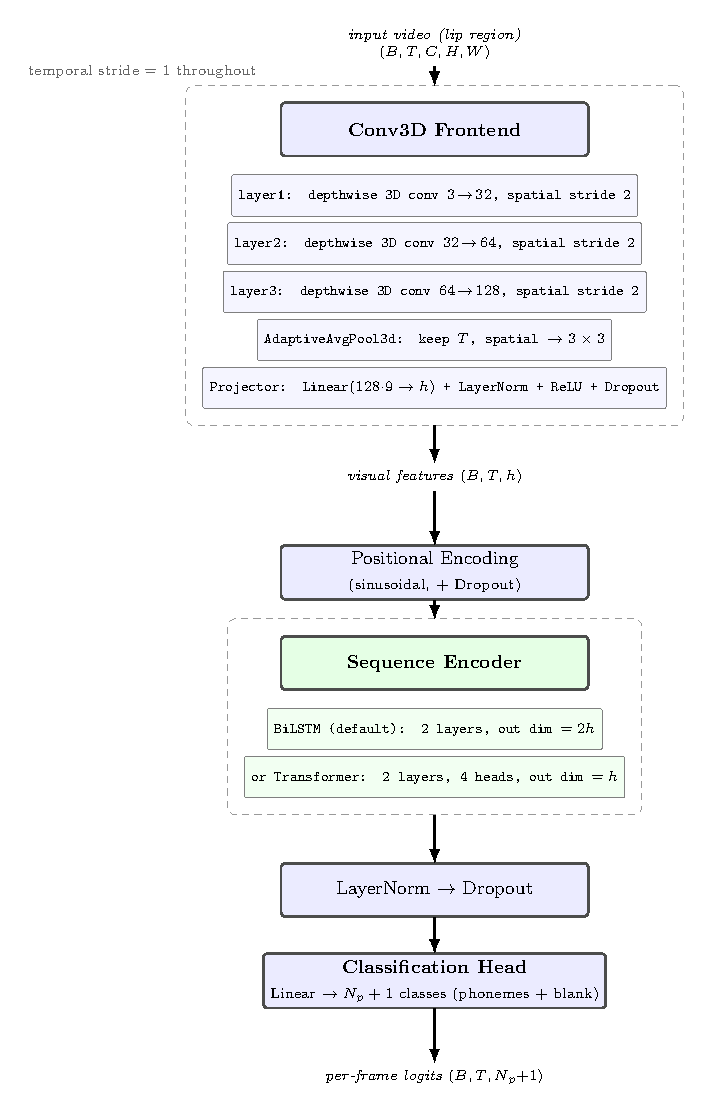
\includegraphics[width=0.8\textwidth]{MethodTikzpic.pdf}
	\caption{Σχηματική παρουσίαση της προτεινόμενης μεθόδου}
	\label{fig:MethodTikzpic}
\end{figure}

\paragraph{Μορφή των δεδομένων εισόδου}

Όσον αφορά τα βίντεο εισόδου, θεωρούμε ότι σε αυτά έχει εφαρμοστεί η πρόβλεψη χειλιών όπως παρουσιάζεται στην παράγραφο \ref{LipExtraction}. Θεωρούμε, επίσης, batch size $B$, αριθμό frames $T$, αριθμό καναλιών $C$, ύψος $H$ και πλάτος $W$ σε pixels, με την τελική μορφή των δεδομένων εισόδου, όπως φαίνεται και στο σχήμα \ref{fig:MethodTikzpic}, να είναι $B \times T \times C \times H \times W$.

\paragraph{Εξαγωγή των Visual Features: Conv3D Frontend}

Η βασική σχεδιαστική επιλογή του συγκεκριμένου μοντέλου είναι η χρήση 3D συνελικτικού νευρωνικού δικτύου ως το πρώτο στάδιο του μοντέλου και όχι διδιάστατου νευρωνικού εφαρμοσμένου σε κάθε frame του βίντεο χωριστά. Η επιλογή αυτή συμβαίνει συνειδητά λόγω της φύσης του προβλήματος του διαβάσματος των χειλιών, το οποίο είναι τόσο πρόβλημα αναγνώρισης της εμφάνισης των χειλιών όσο είναι και πρόβλημα αναγνώρισης των κινήσεών τους. Η διαφοροποίηση μεταξύ πολλών φωνημάτων δεν έγκειται συχνά στην εικόνα απομονωμένων frames όσο στη σχέση μεταξύ διαδοχικών frames, η οποία φανερώνει, για παράδειγμα, την ταχύτητα με την οποία κλείνουν τα χείλη. Η πληροφορία αυτή, αν δεν μαθαίνεται ήδη από τα αρχικά στάδια του μοντέλου, πρέπει να μαθευτεί αποκλειστικά από το επόμενο στάδιο του μοντέλου (τον sequence encoder), ο οποίος σε αυτήν την περίπτωση έχει πρόσβαση μόνο σε στατική περιγραφή κάθε frame ξεχωριστά. Ωστόσο, σε εκείνο το στάδιο υπάρχει και η μακροπρόθεσμη παρακείμενη πληροφορία (πληροφορία που έχει να κάνει με ποια φωνήματα προηγούνται και ποια έπονται), οπότε κρίθηκε χρίσιμο η πληροφορία της κίνησης των χειλιών σε γειτονικά frames να εξάγεται ήδη από τον feature extractor.

Για κάθε ένα από τα 3 blocks συνελικτικού δικτύου 3 διαστάσεων, δεν εφαρμόζεται η τυπική συνέλιξη 3D, αλλά αυτή χωρίζεται σε 2 στάδια: το depthwise stage, κατά το οποίο μία συνέλιξη με kernel $(3, 3, 3)$ εφαρμόζεται ανεξάρτητα σε κάθε κανάλι της εισόδου, και το pointwise stage, που αποτελείται από μία pointwise ($1 \times 1 \times 1$) συνέλιξη η οποία αναμειγνύει τις προηγούμενες εξόδους. Πρόκειται για μία συνήθη παραγοντοποίηση της συνέλιξης σε 3 διαστάσεις και ονομάζεται depthwise separable convolution (συνέλιξη διαχωρίσιμη ως προς το βάθος). Χρησιμοποιείται λόγω της μείωσης του αριθμού των παραμέτρων που προσφέρει. Συγκεκριμένα, έστω μία τυπική 3D συνέλιξη με πυρήνα $(3, 3, 3)$, η οποία οδηγεί $C_i$ κανάλια εισόδου σε $C_o$ κανάλια εξόδου. Το δίκτυο αυτό υπολογίζει το κάθε κανάλι εξόδου ως ένα σταθμισμένο άθροισμα όλων των καναλιών εισόδου και όλων των 27 πιθανών ``χωροχρονικών'' τοποθετήσεων του πυρήνα, χρειάζεται δηλαδή $27 \cdot C_i \cdot C_o$  παραμέτρους και άλλους τόσους πολλαπλασιασμούς και προσθέσεις. Από την άλλη, κατά το depthwise βήμα του depthwise separable convolution, κάθε κανάλι γίνεται αντικείμενο συνέλιξης με τον δικό του πυρήνα $(3, 3, 3)$ χωρίς να αναμειγνύεται με άλλα κανάλια, χρειάζονται δηλαδή $27 \cdot C_i$ παράμετροι. Η μίξη μεταξύ των καναλιών συμβαίνει στο pointwise stage, το οποίο δεν προσφέρει παρακείμενο (context) ούτε στη χρονική ούτε στις χωρικές διαστάσεις και άρα χρειάζεται $C_i \cdot C_o$ παραμέτρους, ίδιες με την περίπτωση fully connected layer μεταξύ των δύο καναλιών. Τελικά, χρησιμοποιώντας τη μέθοδο της depthwise separable convolution, οι απαιτούμενες παράμετροι και πράξεις μειώνονται από $27 \cdot C_i \cdot C_o$ σε $27 \cdot C_i + C_i \cdot C_o$, ελαττώνοντας αισθητά το υπολογιστικό κόστος του μοντέλου.

Πιο συγκεκριμένα, για τα 3 συνελικτικά μπλοκ που χρησιμοποιούνται στο μοντέλο, παρατηρούνται οι εξής μειώσεις σε παραμέτρους: για το πρώτο μπλοκ, ενώ με τυπική 3D συνέλιξη θα υπήρχαν $27\cdot3\cdot32 = 2592$ παράμετροι, ενώ με τη μέθοδο της depthwise separable convolution υπάρχουν $27\cdot3+3\cdot32 = 177$, μείωση δηλαδή κατά πάνω από 93\%. Αντίστοιχα, για το δεύτερο μπλοκ η μείωση είναι από $27\cdot32\cdot64 = 55296$ σε $27\cdot32 + 32\cdot64 = 2912$, δηλαδή σχεδόν 19 φορές, ενώ στο τρίτο μπλοκ οι παράμετροι ελαττώνονται από $27\cdot64\cdot128 = 221184$ σε $27\cdot64 + 64\cdot128 = 9920$, άρα πάνω από 22 φορές λιγότερες. Παρατηρούμε ότι, όσο αυξάνεται το μέγεθος των καναλιών (συγκεκριμένα του καναλιού εξόδου), τόσο μεγαλύτερο γίνεται και το κέρδος χρήσης της μεθόδου αυτής, κάτι που γίνεται προφανές αν συγκριθούν οι όροι $C_i\cdot(27+C_o)$ και $C_i\cdot27\cdot C_o$: ο συντελεστής του $C_i$ στον έναν όρο αυξάνει προσθετικά ενώ στον άλλον πολλαπλασιαστικά με το $C_o$.

Το trade-off της συγκεκριμένης μεθόδου είναι η ενίσχυση του inductive bias (επαγωγική μεροληψία) του μοντέλου: η φύση της depthwise separable convolution υποθέτει ότι τα διάφορα μοτίβα σε χώρο και χρόνο (spatiotemporal patterns) μπορούν να εντοπιστούν σε κάθε κανάλι ξεχωριστά. Η επίδραση του περιορισμού εξαρτάται από το βάθος του δικτύου στο οποίο αναφερόμαστε. Στο πρώτο συνελικτικό μπλοκ, τα κανάλια είναι RGB, με αποτέλεσμα ένα depthwise φίλτρο να είναι ικανό να εντοπίσει ακμές στον χώρο ή αλλαγές στον χρόνο σε κάθε ξεχωριστό κανάλι. Στην περίπτωση του πρώτου μπλοκ, η μόνη περίπτωση που μπορεί να εκφραστεί στην περίπτωση της πλήρους 3D συνέλιξης και όχι της μεθόδου που χρησιμοποιείται είναι ενός φίλτρου που αποκρίνεται διαφορετικά σε κόκκινη ακμή από ότι σε μπλε ακμή ίδιου χρώματος. Αυτή η χρωματική διάκριση δεν αποτελεί αντικείμενο του lip reading, καθώς τα στοιχεία που αναζητώνται (η θέση των χειλιών, η γεωμετρία του ανοίγματος και του κλεισίματός τους και η κίνησή τους) εμφανίζονται ως διαφορές φωτεινότητας και σχήματος που εμφανίζονται σε κάθε κανάλι.

Ο περιορισμός που προκαλείται λόγω αυτού του inductive bias ενισχύεται στα επόμενα μπλοκ συνέλιξης, όπου τα κανάλια δεν είναι πλέον κανάλια χρώματος αλλά feature maps. Σε αντίθεση με τα τυπικά 3D φίλτρα, τα οποία μπορούν να εντοπίσουν σε ένα βήμα την ενεργοποίηση δύο διαφορετικών καναλιών, η μέθοδος αυτή δεν μπορεί να κάνει τη μίξη των καναλιών να εξαρτάται από το χωρικό και χρονικό παρακείμενο εντός ενός block. Έτσι, χάνεται εκφραστικότητα του μοντέλου σε κάθε ξεχωριστή στρώση, η οποία ως έναν βαθμό περιορίζεται λόγω της ύπαρξης και του τελευταίου συνελικτικού μπλοκ, το οποίο μπορεί να εκφράσει κάποια πολυκαναλικά μοτίβα που δεν ήταν δυνατόν να εκφραστούν στην προηγούμενη στρώση. Δεδομένου του μεγέθους των dataset για το πρόβλημα αυτό, ο συμβιβασμός αυτός φαίνεται να αξίζει, καθώς η χαμένη εκφραστικότητα αναπληρώνεται ως ένα σημείο με μεγαλύτερο βάθος, ενώ ταυτόχρονα η βελτίωση στην αποδοτικότητα της εκπαίδευσης είναι πολύ μεγάλη. Η επίδραση της επιλογής αυτής στην ποιότητα της μάθησης δεν εξετάζεται συγκριτικά στην παρούσα εργασία, ενώ η σύγκριση με την πλήρη 3D συνέλιξη αναφέρεται ως πιθανή μελλοντική επέκταση (βλ. ενότητα \ref{Future}).

Τα τρία συνελικτικά μπλοκ αυξάνουν τον αριθμό των καναλιών (από 3 σε 32, 64 και τέλος 128), ενώ κάθε ένα από αυτά έχει χωρικό stride 2, άρα η χωρική ανάλυση μειώνεται κατά 8 φορές. Αντιθέτως, το χρονικό stride είναι 1, έτσι ώστε να μη μειώνεται σε καμία περίπτωση ο αριθμός των frames. Η διατήρηση του αριθμού των frames κάθε βίντεο δεν οφείλεται αποκλειστικά στο βήμα αυτό, αλλά και στο temporal padding με τιμή 1 που εφαρμόζεται: για αριθμό frames εισόδου $T_i$, μήκος padding $p$, μέγεθος kernel $k$ και stride $s$, έχουμε αριθμό frames στην έξοδο του συνελικτικού block $T_o = \lfloor((T_i + 2\cdot p - k) / s) \rfloor + 1$ και τελικά με τις επιλογές που έχουν γίνει $T_o = \lfloor((T_i + 2\cdot 1 - 3) / 1) \rfloor + 1 = T_i$. Χωρίς το padding, κάθε συνελικτικό block μειώνει την αλληλουχία frames κατά 2, κάτι που θα ήταν καταστροφικό για τα labels για κάθε frame που έχουν δημιουργηθεί προηγουμένως. Το kernel με μέγεθος 3, ωστόσο, επιτρέπει στο μοντέλο να μάθει χρονικές εξαρτήσεις προσθέτοντας 2 frames στο receptive field του μοντέλου για κάθε στρώση, δημιουργώντας στην έξοδο του τελευταίου layer ένα receptive field από 7 frames, ικανό να περιγράψει την κίνηση των χειλιών και την παραγωγή των φωνημάτων, όπως και τη μετάβαση μεταξύ τους.

Μετά τα 3 συνελικτικά μπλοκ, χρησιμοποείται pooling μέσω AdaptiveAvgPool3d((None, 3, 3)), περιορίζοντας τις χωρικές διαστάσεις σε έναν σταθερό πίνακα $3\times3$ και διατηρώντας τη χρονική διάσταση σταθερή. Η επιλογή αυτή γίνεται ώστε το μοντέλο να είναι ανεξάρτητο από το μέγεθος του αρχικού βίντεο που εισάγεται σε αυτό. Έτσι, η αρχιτεκτονική μπορεί να εφαρμοστεί για διάφορα μεγέθη crop. Τελικά, τα παραγόμενα διανύσματα σε διάσταση $128\times3\times3 = 1152$ αποτελούν είσοδο σε έναν γραμμικό projector προς την κρυφή διάσταση $h$ (hidden dimension), η οποία έχει την προεπιλεγμένη τιμή 256, μειώνοντας τη διάσταση των δεδομένων προτού εισαχθούν στον sequence encoder. Ακολουθεί η εφαρμογή Layer Normalization, ReLU activation function και Dropout, βελτιώνοντας την κανονικοποίηση του μοντέλου. Οι διαστάσεις των δεδομένων είναι πλέον $(B,T,h)$

\paragraph{Positional Encoding}

Λόγω της πιθανής επιλογής χρήσης transformer αντί για Bi-LSTM στη βαθμίδα του sequence encoding, απαιτείται η χρήση positional encoder, ώστε να υπάρχει πληροφορία της σειράς των feature vectors που παράγονται από το 3D CNN frontend. Χρησιμοποιείται τυπική ημιτονοειδής κωδικοποίηση της θέσης των feature vectors, όπως παρουσιάζεται στην ενότητα \ref{MachineLearningBackground}. Η κωδικοποίηση αυτή, αν και δε χρειάζεται στην περίπτωση χρήσης Bi-LSTM sequence encoder, μια και τα LSTM από τη φύση τους διατηρούν πληροφορία για την αλληλουχία των tokens, διατηρείται και στην περίπτωση επιλογής Bi-LSTM (η οποία είναι η προεπιλογή και είναι αυτή που παρουσιάζεται στο σχήμα \ref{fig:MethodTikzpic}) για συνοχή της αρχιτεκτονικής και ώστε ο encoder να μπορεί να αλλάξει χωρίς να πρέπει να μεταβληθεί το υπόλοιπο pipeline.

\paragraph{Sequence Encoder}

Για την επίτευξη του στόχου του lip reading, είναι σημαντικό να προσαρτηθεί στην τελική απόφαση του μοντέλου μεγαλύτερο παρακείμενο (context), συγκεκριμένα στη διάσταση του χρόνου. Το μοντέλο, έχοντας πρόσβαση σε περισσότερη πληροφορία για το παρελθόν και το μέλλον της ακολουθίας των φωνημάτων, μπορεί να μάθει να εξάγει συμπεράσματα για ένα φώνημα όχι μόνο από τα frames της γειτονιάς στην οποία εκφέρεται, αλλά και από αυτά που προηγήθηκαν ή έπονται. Είναι ευχής έργον το μοντέλο να μάθει εξαρτήσεις φωνημάτων από το παρακείμενο, ιδιαίτερα σε περιπτώσεις όπου το λεξιλόγιο στο οποίο εκπαιδεύεται το μοντέλο είναι περιορισμένο. Ακόμα και σε μη περιορισμένες περιπτώσεις, ωστόσο, ένα μοντέλο δύναται να μάθει γενικές εξαρτήσεις κάποιας γλώσσας (π.χ. ότι στην αγγλική σε παρακείμενο με τη λέξη ``dog'', οι λέξεις ``bark'' ή ``park'' είναι πιο πιθανές από τη λέξη ``mark'' και άρα τα φωνήματα /b/ ή /p/ πρέπει να προβλεφθούν με μεγαλύτερο βάρος από το /m/, παρά το γεγονός ότι οι λέξεις έχουν την ίδια εικόνα στα χείλη) και με βάση αυτές να βελτιώσει τις προβλέψεις του, ειδικά σε περιπτώσεις σύγχυσης σε κάποια κλάση viseme. 

Για τον λόγο αυτόν χρησιμοποείται στο μοντέλο ο Sequence Encoder, δηλαδή ο κωδικοποιητής αλληλουχίας, δουλειά του οποίου είναι να συμπτύξει την πληροφορία του παρακειμένου και οποιουδήποτε δεδομένου token και με βάση αυτά να δημιουργήσει ένα νέο embedding το οποίο αξιοποιεί και τα δύο. Εξετάζονται δύο τύποι sequence encoders (όπως και η εκδοχή με την πλήρη παράλειψή του): ο ένας αξιοποιεί την αρχιτεκτονική των BiLSTMs (bi-directional long-short term memory) και ο άλλος απαρτίζεται από transformers. Η εκδοχή βασισμένη στα BiLSTMs είναι η προεπιλεγμένη και είναι αυτή που παρουσιάζεται στο σχήμα \ref{fig:MethodTikzpic}. Στις παρακάτω παραγράφους παρουσιάζονται και συγκρίνονται αμφότερες οι μέθοδοι.

Η εκδοχή με BiLSTM χρησιμοποιεί 2 στρώσεις της συγκεκριμένης αρχιτεκτονικής, οι οποίες επιτρέπουν στην αναπαράσταση του κάθε frame να επηρεάζεται τόσο από παρελθοντικό όσο και από μελλοντικό παρακείμενο, και παράγει έξοδο με διάσταση $2\cdot h$, διπλασιάζει δηλαδή την κρυφή διάσταση. Στην περίπτωση του transformer χρησιμοποείται multi-head self-attention με προεπιλεγμένη τιμή 4 heads και 2 layers, ενώ η διάσταση εξόδου παραμένει σταθερή και ίση με $h$. Για να μπορούν να συγκριθούν οι δύο εκδοχές, ακολουθούνται και οι 2 από layer normalization και dropout πριν την είσοδο των δεδομένων στην κεφαλή ταξινόμησης.

Σε περίπτωση που τα βίντεο ενός batch έχουν αρχικά διαφορετικό μήκος και άρα τα μικρότερα από αυτά έχουν υποστεί padding, χρησιμοποιούνται για τις δύο εκδοχές του μοντέλου διαφορετικές μέθοδοι για να μην επιτρέπεται στα padded frames να επηρεάζουν την εκπαίδευση. Για το BiLSTM χρησιμοποιούνται τα pack\_padded\_sequence και pad\_packed\_sequence, τα οποία αφαιρούν τα padded frames από τη διαδικασία της αναδρομής. Το μοντέλο που χρησιμοποιεί transformer χρησιμοποιεί μία μάσκα src\_key\_padding\_mask η οποία μηδενίζει το βάρος του attention από και προς padded frames. 

Όσον αφορά τον αριθμό παραμέτρων για κάθε μοντέλο, το BiLSTM αποτελείται από περίπου 2.63 εκατομμύρια παραμέτρους, ενώ ο transformer από 1.58 εκατομμύρια, σχεδόν 1.66 φορές λιγότερες. Αυτό οφείλεται κυρίως στο γεγονός ότι στην έξοδο της πρώτης στρώσης του BiLSTM τα hidden states του προς τα μπροστά και του προς τα πίσω passes συνενώνονται, δημιουργώντας τελικά για τη 2η στρώση είσοδο διάστασης $2\cdot h$ και αυξάνοντας το κόστος της. Οι παράμετροι του transformer παραμένουν ανάλογες με την αρχική κρυφή διάσταση $h$, καθώς δεν υπάρχει μεταβολή ανάμεσα στη διάσταση της εισόδου και της εξόδου τους.

\paragraph{Κεφαλή Ταξινόμησης - Classification Head}

Για να παραχθούν οι τελικές προβλέψεις logits για κάθε frame, χρησιμοποιείται μία γραμμική στρώση η οποία προβάλλει την έξοδο του sequence encoder (με διάσταση $2h$ όταν επιλέγεται το BiLSTM και $h$ όταν χρησιμοποείται ο transformer) στη διάσταση $N_p+1$, όπου $N_p$ είναι η διάσταση του λεξιλογίου που χρησιμοποιείται (ο αριθμός των φωνημάτων που περιλαμβάνονται στη μελέτη ή στο συγκεκριμένο dataset). Η μία διάσταση παραπάνω οφείλεται στην ύπαρξη του κενού/blank συμβόλου, που αντιπροσωπεύει τη σιγή. Και σε αυτό το στάδιο δεν υπάρχει υποδειγματοληψία του χρόνου, ώστε οι προβλέψεις να έχουν το ίδιο μήκος με αυτό της πραγματικής αλληλουχίας φωνημάτων και να έχει νόημα ο υπολογισμός του όρου cross entropy. 

\subsection{Audiovisual Μοντέλο}
\label{AudiovisualModel}
Στην ενότητα αυτή περιγράφεται αναλυτικά η αρχιτεκτονική του προτεινόμενου audiovisual μοντέλου, το οποίο συνδυάζει τόσο το ηχητικό όσο και το σήμα βίντεο για την πρόβλεψη των φωνημάτων. Στα σχήματα \ref{fig:MethodTikzpic2} και \ref{fig:MethodTikzpic3}, παρουσιάζεται μία απεικόνιση των βασικών σχεδιαστικών επιλογών του μοντέλου.

Το μοντέλο αποτελείται από 5 διαδοχικά στάδια:
\begin{enumerate}
\item Τα 2 ανεξάρτητα συνελικτικά frontends, υπεύθυνα για την εξαγωγή των πληροφοριών από το βίντεο και από τον ήχο.
\item Positional Encoding, το οποίο εξυπηρετεί το Cross-Modal Attention που ακολουθεί, όπως και την ύπαρξη της επιλογής του Transformer στο στάδιο του Sequence Encoder.
\item Cross-Modal Attention και στις δύο κατευθύνσεις (audio $\rightarrow$ video και video $\rightarrow$ audio).
\item Συνένωση των αναπαραστάσεων του βίντεο και του ήχου με βάση την αξιοπιστία τους (Reliability-gated fusion)
\item Sequence Encoder με ταξινόμηση σε επίπεδο frame
\end{enumerate}

Για κάθε ένα από τα στάδια αυτά, γίνεται ειδική αναφορά παρακάτω.

\begin{figure}[p]
	\centering
	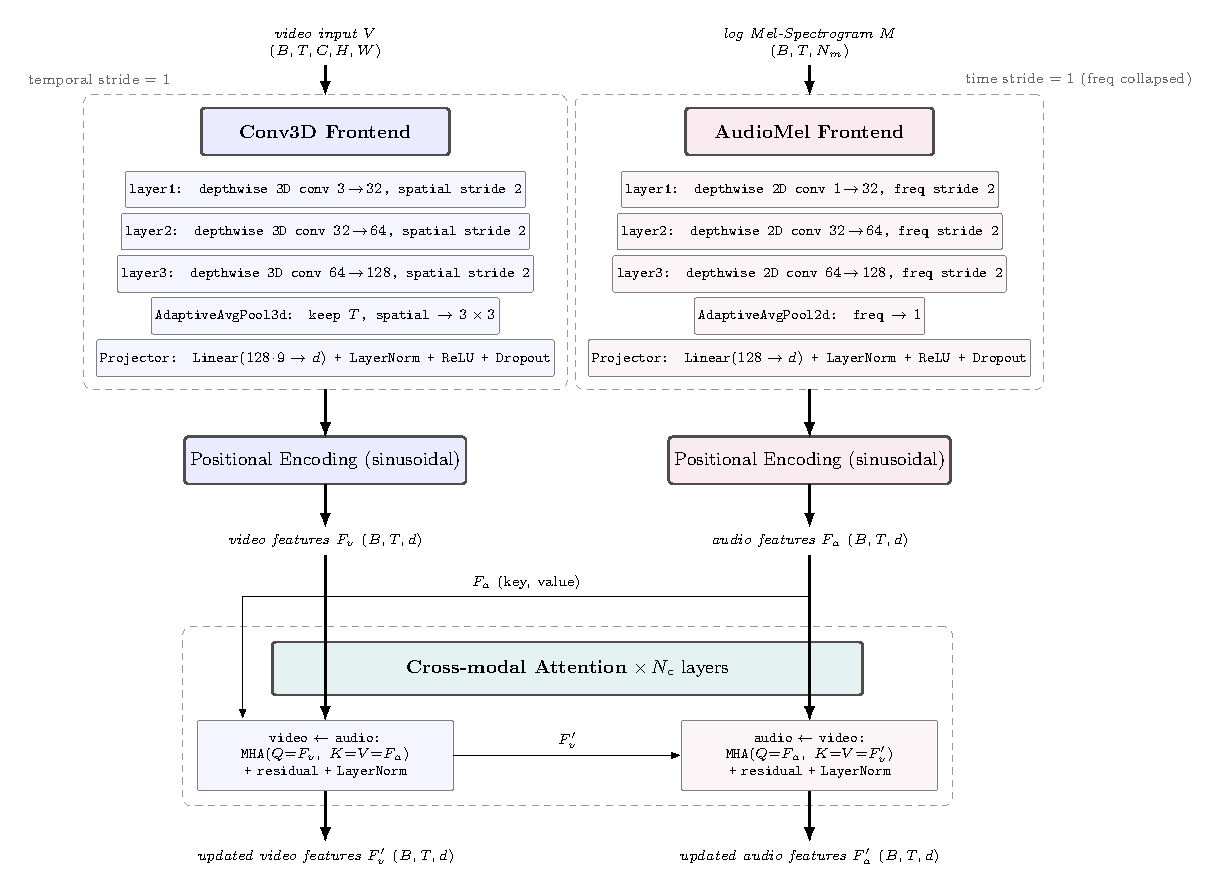
\includegraphics[width=\textwidth]{MethodTikzpic2.pdf}
	\caption{Σχηματική παρουσίαση της προτεινόμενης μεθόδου για το audiovisual model, 1ο σχήμα}
	\label{fig:MethodTikzpic2}
\end{figure}

\begin{figure}[p]
	\centering
	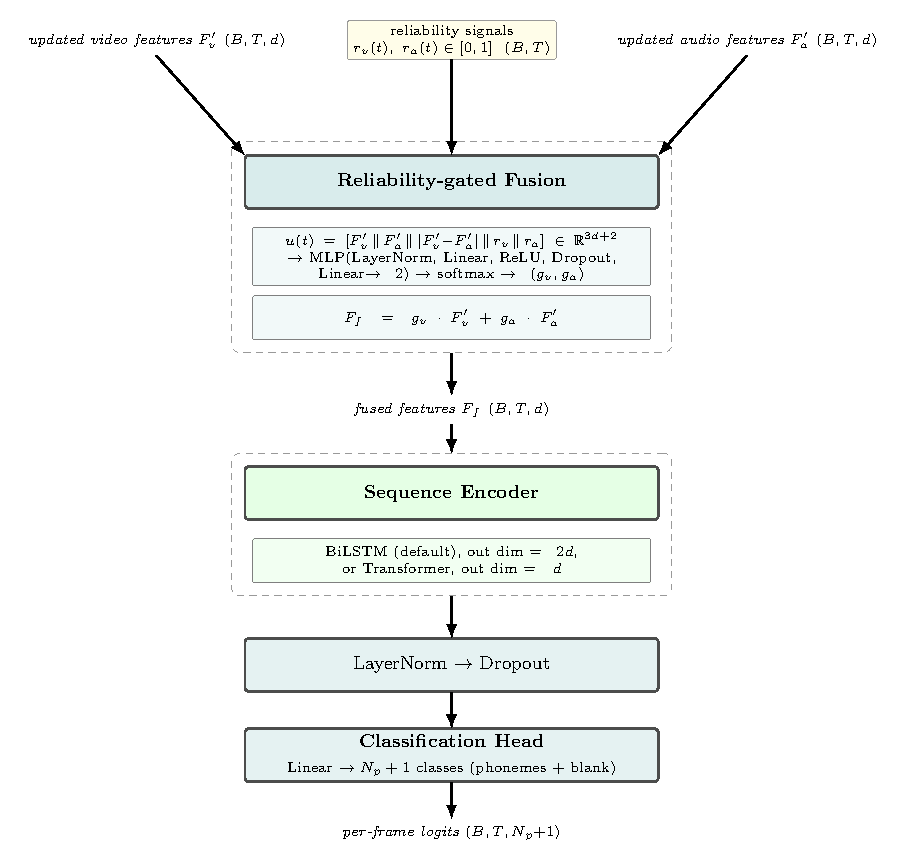
\includegraphics[width=\textwidth]{MethodTikzpic3.pdf}
	\caption{Σχηματική παρουσίαση της προτεινόμενης μεθόδου για το audiovisual model, 2ο σχήμα}
	\label{fig:MethodTikzpic3}
\end{figure}

\paragraph{Δομή των δεδομένων εισόδου}

Κάθε instance εισόδου για το audiovisual μοντέλο αποτελείται από τις εξής χρονικά ευθυγραμμισμένες εισόδους ($t = 1,...,T$):

\begin{itemize}
\item ένα βίντεο $V \in \mathbb{R}^{T \times C \times H \times W}$, όπου $C$ είναι ο αριθμός των καναλιών (3 για βίντεο RGB), $H$ το ύψος και $W$ το πλάτος του κάθε frame σε pixels. Υπενθυμίζεται ότι το βίντεο είναι εστιασμένο στην περιοχή των χειλιών, όπως στην περίπτωση του μοντέλου που αξιοποιεί αποκλειστικά το βίντεο.

\item ένα λογαριθμικό Mel-Spectrogram $M \in \mathbb{R}^{T \times N_m}$, που υπολογίζεται από το αρχικό ηχητικό σήμα σύμφωνα με τα περιεχόμενα της ενότητας \ref{MelSpectrogram}.

\item τα σκορ αξιοπιστίας $r_v(t) \in [0,1]$ και $r_a(t) \in [0,1], t = 1,...,T$ του βίντεο και του ήχου αντίστοιχα για κάθε frame. Υπολογίζονται όπως περιγράφεται στην ενότητα \ref{AudiovisualPreprocessing}. Τα σκορ αυτά θεωρούνται, προς διευκόλυνση του προβλήματος, δεδομένες πληροφορίες και όχι κάτι που πρέπει να υπολογίζεται από το ίδιο το νευρωνικό δίκτυο. Ο τρόπος με τον οποίο χρησιμοποιούνται τα εν λόγω σήματα σχολιάζεται παρακάτω.
\end{itemize}

Για τα παρακάτω, θεωρείται ότι το batch size είναι ίσο με $B$ και ότι τα κανάλια $C$ είναι πράγματι 3, αντικατοπτρίζοντας τη χρήση RGB βίντεο.

\paragraph{Εξαγωγή των Visual Features: Conv3D Frontend}
Το Conv3D Frontend είναι υπεύθυνο για την εξαγωγή των visual features, δηλαδή των χρήσιμων στοιχείων που εμπεριέχονται στο βίντεο. Μετατρέπει τη ροή των δεδομένων του βίντεο από την αρχική διάσταση $V \in \mathbb{R}^{B \times T \times C \times H \times W}$ σε μία αλληλουχία embeddings για κάθε frame της μορφής $F_v \in \mathbb{R}^{B \times T \times d}$, όπου $d$ είναι η κρυφή διάσταση (hidden dimension), με προεπιλεγμένη τιμή 256.

Ως επέκταση της αρχικής προτεινόμενης μεθοδολογίας, η μορφή του Conv3D Frontend είναι πανομοιότυπη με αυτήν του αντίστοιχου block του αρχικού visual μοντέλου. Έτσι, συνεχίζει και στην περίπτωση αυτήν να ισχύει η επιλογή της depthwise 3D συνέλιξης για τη μείωση του υπολογιστικού κόστους, η επιλογή βήματος στον χρονικό άξονα μονίμως 1, ενώ στους χωρικούς άξονες είναι 2 και η γενικότερη μορφή του συνελικτικού δικτύου (με 3 συνελικτικά blocks, αυξάνοντας τον αριθμό των καναλιών από 3 σε 32, μετά σε 64 και τελικά σε 128, ακολουθόμενο από AdaptiveAvgPool3d που κρατά τον χρονικό άξονα αλλά εφαρμόζεται σε περιοχή 3x3 στον χώρο, έπειτα από τον γραμμικό projector, ο οποίος προβάλλει το διάνυσμα feature από την αρχική διάσταση $128 \times 3 \times 3 = 1152$ στη διάσταση $d$ και τέλος από στρώσεις LayerNorm, ReLU και dropout). 

Τελικά, τα δεδομένα έχουν πλέον τη μορφή $F_v \in \mathbb{R}^{B \times T \times d}$, όπου για κάθε βίντεο του batch το κάθε $F_v(t) \in \mathbb{R}^d, t=1,...,T$ αποτελεί την αναπαράσταση των χαρακτηριστικών του βίντεο για το frame $t$. Για περισσότερες λεπτομέρειες αναφορικά με τη λειτουργία του μπλοκ αυτού, όπως και τις διάφορες σχεδιαστικές επιλογές που το απαρτίζουν, ανατρέξτε στην ενότητα \ref{ModelStructure}.

\paragraph{Εξαγωγή των Audio Features: AudioMel Frontend}

Το frontend που χρησιμοποιείται για το ηχητικό σήμα είναι ουσιαστικά το ανάλογο του αντίστοιχου μπλοκ για το βίντεο, στις 2 διαστάσεις αντί για τις 3 (μια και τα Mel-Spectrograms είναι διδιάστατα σήματα και όχι τρισδιάστατα, όπως το βίντεο). Το audio frontend προβάλλει το Mel-Spectrogram $M \in \mathbb{R}^{T \times N_m}$ σε μία σειρά από embeddings (features εξαγόμενα από τον ήχο) $F_a \in \mathbb{R}^{B \times T \times d}$, όπου $d$ είναι και πάλι η κρυφή διάσταση. Εντός του block, εκτελούνται τα ακόλουθα βήματα:

\begin{enumerate}
\item Το φασματογράφημα επιδέχεται reshaping ώστε να αποτελεί μονοκαναλική εικόνα $(B,1,T,N_m)$, όπου οι χωρικοί άξονες είναι αυτοί του χρόνου και των συχνοτήτων mel. Αυτό επιτρέπει την depthwise separable συνέλιξη που ακολουθεί.

\item Ακολουθούν 3 depthwise separable συνελικτικά block, με φίλτρα 3x3, όπου τα κανάλια αυξάνονται από 1 σε 32, έπειτα σε 64 και τέλος σε 128. Κάθε ένα από αυτά χρησιμοποιεί stride 1 στον χρονικό άξονα και 2 στον άξονα των συχνοτήτων mel. Η επιλογή αυτή εξυπηρετεί τη διατήρηση του χρονικού άξονα.

\item Εφαρμόζεται AdaptiveAvgPool2d το οποίο εφαρμόζεται στον άξονα των συχνοτήτων και όχι σε αυτόν του χρόνου, παράγοντας για κάθε frame ένα διάνυσμα χαρακτηριστικών στις 128 διαστάσεις (όσες και τα κανάλια μετά το 3ο συνελικτικό μπλοκ, άρα οι συχνότητες ``καταρρέουν'').

\item Τέλος, εφαρμόζεται μία γραμμική στρώση αξιοποιώντας Layer Normalization, ReLU και Dropout, ακριβώς όπως στην περίπτωση του αντίστοιχου συνελικτικού block της πληροφορίας του βίντεο. Η γραμμική στρώση οδηγεί και πάλι στην κρυφή διάσταση $d$, όπως και στην περίπτωση του βίντεο, ώστε τα τελικά σήματα $F_a(t)$ και $F_v(t)$, τα οποία περιέχουν τα per-frame features του ηχητικού σήματος και του βίντεο αντίστοιχα, να έχουν την ίδια διάσταση.
\end{enumerate}

Το συγκεκριμένο block εκτελεί λειτουργία για το φασματογράφημα των συχνοτήτων mel παρόμοια με αυτήν που εκτελεί ένα συνελικτικό δίκτυο ταξινόμησης για μία εικόνα. Συγκεκριμένα, οι πρώτες στρώσεις, οι οποίες λειτουργούν με μικρό δεκτικό πεδίο (receptive field) εντός του επιπέδου χρόνου-συχνοτήτων, μαθαίνουν βασικά τοπικά πρότυπα (patterns) της αναπαράστασης της ομιλίας σε φασματογράφημα (όπως, για παράδειγμα, την τοπική εμφάνιση των διάφορων formants - των βασικών συχνοτητών κατά την ομιλία - ή τη μεταφορά από έμφωνα σε άφωνα τμήματα της ομιλίας). Οι βαθύτερες στρώσεις συνδυάζουν τα τοπικά συμπεράσματα των προηγούμενων στρώσεων και εξάγουν μία γενικότερη αναπαράσταση του κάθε βήματος χρόνου, η οποία μπορεί να χρησιμοποιηθεί για την τελική πρόβλεψη φωνημάτων. Έτσι, οι μετέπειτα στρώσεις ανταποκρίνονται και σε πρότυπα σε μεγάλη περιοχή του φάσματος, όπως την απεικόνιση των formants που διαχωρίζει τα φωνήεντα, και δεν περιορίζονται σε μόνο τοπικά bins συχνοτήτων, ιδιότητα η οποία είναι βασική για την ορθή πρόβλεψη φωνημάτων.

Επιλέγεται και για αυτό το block η depthwise separable συνέλιξη αντί για την τυπική εκδοχή της. Η 2D συνέλιξη χωρίζεται πρώτα σε ένα depthwise βήμα (ένα φίλτρο 3x3 για κάθε κανάλι, χωρίς μίξη μεταξύ των καναλιών), το οποίο ακολουθείται από ένα pointwise βήμα 1x1 κατά το οποίο αναμειγνύεται η πληροφορία των καναλιών. Ο διαχωρισμός αυτός μειώνει τον αριθμό των παραμέτρων του κάθε συνελικτικού τμήματος (για λόγους πλήρως όμοιους με αυτούς του αντίστοιχου βίντεο block, όπως φαίνεται στην ενότητα \ref{ModelStructure}) από $O(k^2 \cdot C_i \cdot C_o)$ σε $O(k^2 \cdot C_i + C_i \cdot C_o)$, όπου $k$ είναι το μέγεθος του πυρήνα (εδώ 3) και $C_i, C_o$ είναι ο αριθμός των καναλιών της εισόδου και της εξόδου αντίστοιχα. Η επιλογή αυτή βοηθά αφενός με τη μείωση των παραμέτρων του μοντέλου που εκπαιδεύεται, ενώ ταυτόχρονα διατηρεί συμμετρική τη μορφή των 2 αρχικών feature extractors, για βίντεο και ήχο. Η επιλογή αυτή καθιστά τους 2 feature extractors όμοια εκφραστικούς, αντί ο ένας από τους δύο να έχει μεγαλύτερη εκφραστική δυνατότητα. Μία ασυμμετρία στην εκφραστική ικανότητα θα μπορούσε να προσφέρει ένα bias στις μετέπειτα στρώσεις του μοντέλου, ώστε να εμπιστεύονται κυρίως την τροπικότητα που περιγράφεται με υψηλότερη ικανότητα και όχι αναγκαστικά αυτήν που περιέχει τη λιγότερο θορυβώδη πληροφορία (και άρα είναι πιο αξιόπιστη).

Καθώς το πρόβλημα είναι sequence labelling και όχι πρόβλημα ταξινόμησης ολόκληρης της φράσης, ο χρονικός άξονας πρέπει να διατηρηθεί και στο ηχητικό σήμα (όπως και σε αυτό του βίντεο). Έτσι, όπως προαναφέρθηκε, επιλέγεται stride 2 στον χώρο των συχνοτήτων και 1 σε αυτό του χρόνου, ώστε να μην υπάρχει κατάρρευση του χρονικού άξονα, ο οποίος έχει ευθυγραμμιστεί για τις 2 τροπικότητες και το target phoneme sequence εκ των προτέρων. Αποφεύγεται, με αυτόν τον τρόπο, η ανάγκη χρήσης εργαλείου resampling στον χρόνο, όπως upsampling ή παρεμβολής, πριν τη χρήση των feature vectors $F_a$ και $F_v$ για την εξαγωγή συνολικών συμπερασμάτων με βάση και τις 2 τροπικότητες.

Μία ακόμα ενδιαφέρουσα επιλογή είναι η επιλογή να μην κρατηθεί μία μικρή διάσταση συχνοτητών κατά το pooling (π.χ. να υπάρχει ένας χάρτης χαρακτηριστικών 128x4 για κάθε frame, ο οποίος να προβάλλεται από τη γραμμική στρώση στην κρυφή διάσταση, αντί οι συχνότητες να καταρρέουν τελείως, με τρόπο ανάλογο που γίνεται στην περίπτωση του βίντεο, όπου παραμένει μία περιοχή 3x3 μετά το pooling). Η επιλογή αυτή είναι συνειδητή, καθώς η πληροφορία των δύο σημάτων είναι εν γένει διαφορετική: στο βίντεο, η γενική πληροφορία της θέσης που εντοπίζεται ένα πρότυπο είναι σημαντική για την ομιλία (π.χ. πάνω ή κάτω χείλος), κάνοντας τη διατήρηση μίας μικρής περιοχής χρήσιμη. Αντίθετα, στο Mel-Spectrogram, η πληροφορία κρύβεται στο γενικό σχήμα του συχνοτικού περιεχομένου και όχι στην ακριβή περιοχή που συμβαίνει αυτή η ενεργοποίηση. Έτσι, κρίθηκε εύστοχη απλοποίηση η πλήρης κατάρρευση του άξονα των συχνοτήτων, πριν δοθεί η πληροφορία στη γραμμική στρώση.

Το AudioMel Frontend, όντας αρχιτεκτονικά παρόμοιο με το αντίστοιχο Conv3D Visual Frontend, περιέχει και παρόμοια γραμμική στρώση που παράγει τα τελικά audio features $F_a$. Η επιλογή αυτή δεν είναι τυχαία, καθώς ακολουθεί cross-attention το οποίο υπολογίζει εσωτερικά γινόμενα και αθροίσματα των $F_v(t)$ και $F_a(t)$. Έτσι, τα δύο αυτά σήματα πρέπει να βρίσκονται στην ίδια διάσταση και να χαρακτηρίζονται από παρόμοια κανονικοποίηση. Η επιλογή της αρχιτεκτονικά όμοιας γραμμικής στρώσης για το ηχητικό σήμα έχει ως αποτέλεσμα τη μη εμφάνιση ασυμμετριών προτού ``συναναστραφούν'' τα δύο σήματα, άρα οι ασυμμετρίες που εμφανίζονται τελικά μεταξύ των δύο (π.χ. στις πύλες αξιοπιστίας - reliability gates- που περιγράφονται παρακάτω) να οφείλονται αποκλειστικά στην αξιοπιστία του εκάστοτε σήματος και όχι σε προηγούμενη ανεπάρκεια ενός εκ των δύο εξαγωγέων χαρακτηριστικών.

\paragraph{Positional Encoding}
Προστίθεται στα σήματα $F_v$ και $F_a$ ημιτονοειδές positional encoding (όπως ακριβώς και στην περίπτωση του visual μοντέλου της ενότητας \ref{ModelStructure}), το οποίο είναι ίδιο για κάθε τροπικότητα, πριν την αλληλεπίδραση των δύο. Η επιλογή αυτή είναι αναγκαία για την πλήρη αξιοποίηση της στρώσης Cross-Attention που ακολουθεί (και της επιλογής τελικού transformer encoder), έτσι ώστε να παρέχεται στο μοντέλο πληροφορία περί της χρονικής απόστασης των features του κάθε frame. Χρησιμοποιείται τυπική ημιτονοειδής κωδικοποίηση της θέσης των feature vectors, όπως παρουσιάζεται στην ενότητα \ref{MachineLearningBackground}.

\paragraph{Cross-modal Attention}
Η βασική σχεδιαστική επιλογή υπεύθυνη για την ανάμειξη των πληροφοριών των δύο τροπικοτήτων είναι αυτή του Cross-modal Attention που επιβάλλεται για $N_c$ στρώσεις (με προεπιλεγμένη τιμή $N_c = 1$), πριν το βήμα fusion που συνενώνει τις πληροφορίες πλήρως. Οι είσοδοι στο συγκεκριμένο block είναι οι έξοδοι των Frontends κάθε τροπικότητας, δηλαδή η αλληλουχία χαρακτηριστικών βίντεο $F_v \in \mathbb{R}^{B \times T \times d}$ και η αντίστοιχη αλληλουχία για τον ήχο $F_a \in \mathbb{R}^{B \times T \times d}$. Ο μηχανισμός της Cross-modal Attention λειτουργεί ως εξής:

\begin{enumerate}
\item Πρώτα, εκτελείται Multi-head Attention (MHA) με κατεύθυνση video $\leftarrow$ audio, όπου δηλαδή τα χαρακτηριστικά του video είναι το query, ενώ τα χαρακτηριστικά του audio είναι το key και το value.

\[
\tilde F_v = \operatorname{MHA}_{v \leftarrow a}(Q = F_v, K = F_a, V = F_a)
\]

\item Ακολουθείται Residual Connection και Layer Normalization για τα video features.

\[
F_v\sp{\prime} = \operatorname{LayerNorm}(F_v + \tilde F_v)
\]

\item Έπεται η αντίστροφη Multi-head Attention με κατεύθυνση audio $\leftarrow$ video, όπου τα χαρακτηριστικά του audio είναι το query, ενώ τα χαρακτηριστικά του video είναι το key και το value.

\[
\tilde F_a = \operatorname{MHA}_{a \leftarrow v}(Q = F_a, K = F_v\sp{\prime}, V = F_v\sp{\prime})
\]

\item Τέλος, εφαρμόζεται Residual Connection και Layer Normalization για τα audio features.

\[
F_a\sp{\prime} = \operatorname{LayerNorm}(F_a + \tilde F_a)
\]
\end{enumerate}

Παρακάτω επεξηγούνται μερικές από τις επιλογές που οδήγησαν στην παραπάνω εικόνα.

Ένα σημαντικό ερώτημα είναι γιατί επιλέγεται ο μηχανισμός του Cross-modal Attention και όχι, π.χ. παρεμβολή των features με σταθερά βάρη. Η απάντηση σε αυτό το ερώτημα έγκειται στην ύπαρξη τυχαιοποιημένου θορύβου, ο οποίος όμως είναι σε συνεχόμενα χρονικά σημεία (π.χ. μία αλληλουχία θολών frames ή ένα σημείο που έχει κοπεί ο ήχος). Χρησιμοποιώντας σταθερά βάρη και υπολογίζοντας τη γραμμική παρεμβολή των δύο εξαγόμενων features, το μοντέλο δε συνυπολογίζει ποια από τις δύο τροπικότητες είναι αξιόπιστη για κάθε χρονική στιγμή (και, ακόμα και αν τα βάρη μαθαίνονται, έχει bias προς τη γενικά πιο αξιόπιστη τροπικότητα, αγνοώντας την τοπική πληροφορία). Αντίθετα, ο μηχανισμός attention επιτρέπει σε κάθε frame από κάθε τροπικότητα να αντλήσει τις απαιτούμενες πληροφορίες από κάθε χρήσιμο frame της άλλης τροπικότητας (και όχι αποκλειστικά από το ίδιο frame), δίνοντας την ελευθερία στο μοντέλο να αξιοποιήσει περισσότερο τα χρήσιμα και αξιόπιστα frames ώστε να επηρεαστούν κατάλληλα τα features του audio και του video.

Η cross-modal attention πρέπει να γίνεται προς και τις δύο κατευθύνσεις, δηλαδή audio $\leftarrow$ video αλλά και video $\leftarrow$ audio. Ο λόγος είναι ότι, αν μόνο μία από τις δύο κατευθύνσεις ολοκληρωνόταν, τότε θα δημιουργόταν το bias ότι μόνο μία από τις δύο τροπικότητες θα είχε την ευκαιρία να αντλήσει πληροφορία από την άλλη (π.χ. μόνο η απεικόνιση του ήχου θα αξιοποιούσε αυτήν του βίντεο για να επιδιορθώσει λανθασμένα χαρακτηριστικά που οφείλονται στην ύπαρξη θορύβου). Εφ' όσον οι δύο τροπικότητες επηρεάζονται από τον θόρυβο με ανεξάρτητο και απρόβλεπτο τρόπο, ο μηχανισμός του cross-modal attention πρέπει να εφαρμοστεί προς και τις δύο κατευθύνσεις, ώστε οποιαδήποτε από τις δύο τροπικότητες να μπορεί να βοηθήσει την άλλη, ανάλογα με το ποια από τις δύο αντιμετωπίζει θόρυβο τη συγκεκριμένη χρονική περίοδο (για παράδειγμα, στα σημεία που εφαρμόζεται το θόλωμα στο βίντεο, οι πληροφορίες εξαγόμενες από τον ήχο μπορούν να βελτιώσουν αυτές που εξάγονται από το θορυβώδες βίντεο).

Τέλος, η χρήση της Residual σύνδεσης εξασφαλίζει ότι, αν η cross-modal πληροφορία δεν είναι χρήσιμη για ένα frame (π.χ. επειδή η άλλη τροπικότητα είναι επηρεασμένη βαθιά από τον θόρυβο εκείνη τη στιγμή, ενώ από την αρχική τροπικότητα έχουν εξαχθεί ισχυρά features), τότε δε θα καταστραφεί πλήρως η unimodal αναπαράσταση από την εφαρμογή attention. Η Layer Normalization σταθεροποιεί τα τελικά features $F_v\sp{\prime}$ και $F_a\sp{\prime}$, προτού αυτά εισαχθούν στη fusion gate.

\paragraph{Reliability-gated Fusion}
\label{ReliabilityFusion}
Το block του Reliability-gated Fusion είναι αυτό που τελικά συνδυάζει τις πληροφορίες από τις δύο τροπικότητες και παράγει ένα ολικό feature sequence, αξιοποιώντας τόσο τις αναπαραστάσεις του ήχου $F_a\sp{\prime}(t) \in \mathbb{R}^d$ και του βίντεο $F_v\sp{\prime}(t) \in \mathbb{R}^d$ για κάθε frame, όσο και τα σήματα αξιοπιστίας των δύο τροπικοτήτων $r_a(t), r_v(t) \in [0,1]$, για ήχο και βίντεο αντίστοιχα, στα οποία γίνεται αναφορά στην αρχή της συγκεκριμένης ενότητας.

Ο μηχανισμός του σταδίου αυτού λειτουργεί ως εξής:

\begin{enumerate}
\item Παράγεται ένα διάνυσμα εισόδου $u(t)$ για κάθε frame $t$ ως αποτέλεσμα της παρακάτω συνένωσης (concatenation)
\[
u(t) = [ F_v\sp{\prime}(t) || F_a\sp{\prime}(t) || \lvert F_v\sp{\prime}(t) - F_a\sp{\prime}(t) \rvert || r_v(t) || r_a(t) ] \in \mathbb{R}^{3d+2}
\]

\item Το διάνυσμα αυτό γίνεται η είσοδος σε ένα μικρό δίκτυο MLP (LayerNorm $\rightarrow$ Linear $\rightarrow$ ReLU $\rightarrow$ Dropout $\rightarrow$ Linear), παράγοντας δύο logits, τα οποία κανονικοποιούνται με συνάρτηση softmax στην τελική τους μορφή $(g_v(t),g_a(t))$ με $g_v(t) + g_a(t) = 1$.

\item Υπολογίζεται η συνδυασμένη αναπαράσταση $F_f(t)$ για κάθε frame $t$ ως:
\[
F_f(t) = g_v(t) \cdot F_v\sp{\prime}(t) + g_a(t) \cdot F_a\sp{\prime}(t)
\]
\end{enumerate}

Παράγεται, τελικά, η ακολουθία των συνδυασμένων αναπαραστάσεων $F_f \in \mathbb{R}^{B \times T \times d}$. Η λογική της χρήσης της απόλυτης διαφοράς $\lvert F_v\sp{\prime}(t) - F_a\sp{\prime}(t) \rvert$ έγκειται στο ότι δίνεται στο μοντέλο ένα σήμα που εκφράζει εγγενώς την ασυμφωνία των δύο τροπικοτήτων (η διαφορά αυτή παίρνει μεγάλες τιμές όταν οι δύο τροπικότητες περιέχουν διαφορετικό φωνητικό περιεχόμενο, και άρα κάποια από τις δύο έχει πιθανότατα επηρεαστεί από τον θόρυβο). Χρησιμοποιείται, δηλαδή, ως ένα περαιτέρω σήμα ώστε, σε περίπτωση ύπαρξης θορύβου που επηρεάζει μία από τις δύο τροπικότητες σημαντικά, να μπορεί το μοντέλο να αναγνωρίσει αυτήν τη συμπεριφορά και να αξιοποιήσει περισσότερο την τροπικότητα που έχει επηρεαστεί λιγότερο από τον θόρυβο. Να σημειωθεί ότι η επίδραση του όρου $\lvert F_v\sp{\prime}(t) - F_a\sp{\prime}(t) \rvert$ στην επίδοση του μοντέλου δε μελετάται στην παρούσα εργασία. Ο όρος αυτός, που υπολογίζεται ως η απόλυτη τιμή της διαφοράς ανά στοιχείο (element-wise) των δύο διανυσμάτων και έχει επομένως διάσταση $d$, συμπεριλαμβάνεται απλώς ως μέτρο της διαφοράς των δύο αναπαραστάσεων. Η συγκριτική αξιολόγηση διαφορετικών επιλογών για την είσοδο του σταδίου αυτού αναφέρεται ως μελλοντική επέκταση (βλ. ενότητα \ref{Future}). Σε ένα τελικό σύστημα, έτοιμο να χρησιμοποιηθεί με in the wild θορυβώδη δεδομένα, προφανώς τα σήματα αξιοπιστίας $r_a(t)$ και $r_v(t)$ δε θα ήταν δεδομένα, αλλά θα έπρεπε να υπολογίζονται σε πραγματικό χρόνο από το μοντέλο. Ωστόσο, για απλοποίηση του προβλήματος και κυρίως ως proof of concept, επιλέχθηκε τα σήματα αυτά να είναι διαθέσιμα στο μοντέλο (υπολογισμένα όπως αναγράφεται στην ενότητα \ref{AudiovisualPreprocessing}) και όχι να πρέπει να υπολογίζονται από το μοντέλο.

\paragraph{Sequence Encoder}
Ο Sequence Encoder του μοντέλου αυτού δέχεται ως είσοδο τη συνδυασμένη αναπαράσταση $F_f \in \mathbb{R}^{B \times T \times d}$ και έχει μορφή πλήρως πανομοιότυπη με αυτήν που χρησιμοποιείται στο visual μοντέλο και παρουσιάζεται στην ενότητα \ref{ModelStructure}. Δίνεται και πάλι η επιλογή χρήσης είτε BiLSTM (που είναι και η προεπιλεγμένη εκδοχή), με διάσταση εξόδου $2d$, είτε Transformer με διάσταση εξόδου $d$. Η έξοδος του Sequence Encoder κανονικοποιείται με χρήση LayerNorm, περνά από Dropout και προβάλλεται μέσω μίας τελευταίας γραμμικής στρώσης σε $N_p+1$ logits ανά frame (όπου $N_p$ είναι το μήκος του λεξιλογίου και το $+1$ οφείλεται στην ύπαρξη του blank token του CTC).

\paragraph{Εκτέλεση με μοναδική τροπικότητα}
\label{SingleModality}
Παρέχεται η δυνατότητα εκπαίδευσης μοντέλου που αξιοποιεί μονάχα μία από τις δύο τροπικότητες (είτε μόνο το βίντεο είτε μόνο τον ήχο). Στην περίπτωση αυτή προσπερνώνται τα blocks του cross-attention και του fusion και οι αναπαραστάσεις που παράγονται από την επιλεγμένη τροπικότητα εισέρχονται απ'ευθείας στον sequence encoder.

\subsection{Βήματα Post-Processing}
\label{PostProcessing}

Όπως παρουσιάστηκε το μοντέλο μέχρι τώρα, είναι ικανό μόνο να προβλέψει φωνήματα από το βουβό βίντεο. Στη συγκεκριμένη υποενότητα, περιγράφονται οι τεχνικές post-processing που εφαρμόστηκαν ώστε η αλληλουχία φωνημάτων να μετατραπεί σε λέξεις, βήμα το οποίο οδηγεί στην επίτευξη του πρωταρχικού στόχου του lip reading.

\subsubsection{Αλγοριθμική Πρόβλεψη Λέξεων}
\label{WordPrediction}

Σε εφαρμογές σε περιορισμένο περιβάλλον, όπου το λεξιλόγιο και, προαιρετικά, η γραμματική των φράσεων είναι γνωστά, είναι δυνατόν η πρόβλεψη των λέξεων από την αλληλουχία φωνημάτων να γίνει αλγοριθμικά και χωρίς τη χρήση τεχνητής νοημοσύνης. Για τα παρακάτω, υποθέτουμε (χωρίς βλάβη της γενικότητας και για να γίνει πιο ξεκάθαρη η επεξήγηση της μεθόδου) ότι η ανάλυση γίνεται στο dataset GRID, όπως παρουσιάζεται στην παράγραφο \ref{Datasets}.

Αρχικά, παράγεται το collapsed sequence φωνημάτων από την αλληλουχία των φωνημάτων που προβλέπεται, ενώνοντας γειτονικά ίδια tokens και απαλείφοντας τα blank tokens, δημιουργώντας μία ομάδα από φωνήματα και τους χρονισμούς τους. Έπειτα, χρησιμοποιείται αλγόριθμος δυναμικού προγραμματισμού ώστε να βρεθεί η τομή των φωνημάτων σε λέξεις και η ανάθεση των προβλεπόμενων λέξεων με το μικρότερο συνολικό κόστος. 

Για κάθε υποψήφια λέξη σε κάθε θέση, υπολογίζεται μία τιμή ομοιότητας με την ακολουθία των φωνημάτων που προβλέπεται. Έστω $O$ η πρόβλεψη και $T$ η υποψήφια λέξη. Ορίζεται η βασική απόσταση ως $D(O,T) = \frac{1}{\max(|O|, |T|)} \cdot E(O,T)$, όπου $E(O,T)$ είναι η ελάχιστη απόσταση edit της αλληλουχίας φωνημάτων $O$ ώστε να φτάσει στην $T$. Κάθε φώνημα που πρέπει να αλλαχθεί δεν επηρεάζει με ίδιο τρόπο την $E(O,T)$. Συγκεκριμένα, όμοια φωνήματα (είτε ακουστικά είτε οπτικά) τιμωρούνται λιγότερο σε σχέση με τελείως διαφορετικά φωνήματα. Το κόστος κάθε αλλαγής, από φώνημα $a$ σε φώνημα $b$, υπολογίζεται ως εξής:

$c(a,b) = \begin{cases}
0 & a = b \\
0.15 & \text{ίδια κλάση viseme και ίδιος τρόπος/τόπος εκφοράς, αλλά διαφορετική φω\-νο\-ποί\-η\-ση} \\
0.35 & \text{ίδια κλάση viseme αλλά όχι μόνο διαφορετική φωνοποίηση} \\
\min(1, \frac{\Delta (a,b)}{4}) & \text{αλλιώς, με διαφορά ιδιοτήτων $\Delta$} \\
1 & \text{αν δεν υπάρχει καμία ίδια ιδιότητα}
\end{cases}
$

Τότε, το τελικό σκορ ομοιότητας για κάθε υποψήφια λέξη είναι $S(O,T) = D(O,T) - \beta_a(O,T) -0.15 \beta_r(O,T)$, όπου $\beta_a$ είναι ένα ισχυρό bonus που δίνεται σε φωνήματα anchor και $\beta_r$ είναι ένα μικρότερο bonus για σπάνια φωνήματα. Τα φωνήματα anchor είναι φωνήματα που εμφανίζονται μόνο σε μία υποψήφια λέξη κάποιας κατηγορίας. Για παράδειγμα, στις προθέσεις του GRID, το φώνημα /ð/ με ήχο σαν το ελληνικό θήτα εμφανίζεται μόνο στη λέξη with και όχι σε οποιαδήποτε από τις in, by και at. Εάν δεν υπήρχε αυτός ο όρος, μία αλληλουχία φωνημάτων /i/ /ð/ θα οδηγούσε σε πρόβλεψη in και όχι σε πρόβλεψη with, που φαίνεται πιο αληθοφανές, δεδομένου ότι προβλέφθηκε το /ð/ που ανήκει μόνο σε μία λέξη. Με παρόμοιο τρόπο υπολογίζεται και το $\beta_r$, αλλά πολλαπλασιάζεται με παράγοντα ανάλογο της σπανιότητας του εκάστοτε φωνήματος.

Με την παραπάνω μέθοδο, είναι δυνατόν να προβλεφθούν και λέξεις εντός του περιορισμένου περιβάλλοντος, πέραν των φωνημάτων. Ο αλγόριθμος αυτός σίγουρα μπορεί να αποτελέσει αντικείμενο βελτίωσης και καλύτερης προσαρμογής στο δεδομένο περιβάλλον στο οποίο γίνεται η κάθε μελέτη, ωστόσο κρίθηκε ότι η τωρινή εκδοχή του είναι αρκετή ώστε να επιδείξει ικανοποιητικά αποτελέσματα. Προφανώς, τα παραπάνω δεν μπορούν να εφαρμοστούν σε μη περιορισμένο περιβάλλον, στο οποίο τόσο το λεξιλόγιο όσο και η γραμματική είναι σαφώς πιο ποικιλόμορφα, καθώς η λογική ιδιαίτερα του δυναμικού προγραμματισμού καταρρέει όσο αυξάνεται η πολυπλοκότητα των πιθανών λέξεων και της τοποθέτησής τους.

\subsubsection{Πρόβλεψη Φράσεων από Αλληλουχία Φωνημάτων μέσω LLM}
\label{PhrasePrediction}
Σε περιπτώσεις μη περιορισμένου περιβάλλοντος (in the wild), η αλγοριθμική πρόβλεψη λέξεων από τα φωνήματα είναι προφανώς αδύνατη, λόγω της ύπαρξης μεγάλου αριθμού υποψήφιων λέξεων (ουσιαστικά όλες της αγγλικής - ή οποιασδήποτε άλλης - γλώσσας). Έτσι, απαιτείται ένας διαφορετικός τρόπος ώστε τα φωνήματα που έχουν προβλεφθεί από το μοντέλο να πάρουν μία γλωσσική μορφή που έχει νόημα (δηλ. λέξεις και τελικά φράσεις). Μία μεθοδολογία επίλυσης του συγκεκριμένου προβλήματος που προτείνεται και στο \cite{thomas2026vallrvisualasrlanguage} είναι η ανακατασκευή προτάσεων με χρήση LLM (Large Language Model), fine-tuned για το εν λόγω task (βλ. ενότητα \ref{LLMFineTuning}).

Στη φάση του inference, ζητείται από το LLM με κατάλληλο prompt να παράξει την προβλεπόμενη πρόταση $\hat S$ από την προβλεπόμενη αλληλουχία φωνημάτων $\hat P$. Η μέθοδος αυτή, καθώς αφορά το μη περιορισμένο περιβάλλον, δεν υλοποιήθηκε στο πλαίσιο της παρούσας εργασίας και αποτελεί μία από τις μελλοντικές επεκτάσεις (βλ. ενότητα \ref{Future}).
